\documentclass[aspectratio=169]{beamer}
\usetheme[progressbar=none]{metropolis}           % Use metropolis theme
%\input{metropolis-settings.tex}
\usepackage[T1]{fontenc}
\usepackage[italian]{babel}
\usepackage[sfdefault]{FiraSans}
\usepackage{graphicx}
\graphicspath{{../img/}}

\title{Algoritmo di tagging di raggi cosmici\\in un sistema di acquisizione triggerless\\\mbox{per un esperimento di fisica di particelle su fascio}}
\date{Anno Accademico 2022/2023}
\author{Antonio Ghinassi}
\institute{Corso di Laurea in Fisica $\cdot$ Università di Bologna}

\begin{document}
  \maketitle
  \setbeamertemplate{frame footer}{\insertauthor\hspace{2.6cm}\insertinstitute}%Corso di Laurea in Fisica $\cdot$ Università di Bologna}%Alma Mater Studiorum $\cdot$ Università di Bologna}
  %\section{First Section}
  %SLIDE 1
  \begin{frame}{TriDAS (Triggerless Data Acquisition System)}
      \begin{columns}[onlytextwidth,T]
      \begin{column}{.45\linewidth}
      \begin{itemize}
         \item Acquisizione triggerless
             \begin{itemize}
                \item Implementazione solo software del trigger
                \item Permette criteri più complessi di selezione dei dati
             \end{itemize}
         \item Design modulare e scalabile
             \begin{itemize}
                 \item Moduli scritti in \texttt{C++11}
                 \item Sistema distribuito su più nodi 
             \end{itemize}
         \item Progettato e implementato per KM3NeT, adattato per esperimenti su fascio di particelle
      \end{itemize}
      \end{column}
      \begin{column}{.45\linewidth}
      \end{column}
    \end{columns}
    \begin{tikzpicture}[remember picture, overlay]
    \node[left=0.8cm] at (current page.east) 
    {
        \includegraphics[width=0.45\textwidth]{tridas_scheme_vertical_stripped.png}
    };
    \end{tikzpicture}
  \end{frame}
  %
  \begin{frame}{TriDAS (Triggerless Data Acquisition System)}
    \begin{tikzpicture}[remember picture, overlay]
    \node[right=0.8cm] at (current page.west) 
    {
        \includegraphics[width=0.55\textwidth]{hm_emph.png}
    };
    \end{tikzpicture}
    \begin{tikzpicture}[remember picture, overlay]
    \node[left=0.8cm] at (current page.east) 
    {
        \includegraphics[width=0.45\textwidth]{tridas_scheme_vertical_stripped_emph.png}
    };
    \end{tikzpicture}
  \end{frame}
  %
  \begin{frame}{TriDAS per Clas12 e EIC}
      \begin{columns}[onlytextwidth,T]
      \begin{column}{.60\linewidth}
      \begin{itemize}
          \item Clas12 (CEBAF Large Acceptance Spectrometer for operations at 12 GeV beam energy)
             \begin{itemize}
                \item Studia reazioni adroniche e nucleari indotte dalla collisione di elettroni
                %\item In grado di distinguere elettroni diffusi e adroni prodotti dalle collisioni su un ampio angolo solido
                \item Opera a luminosità di \SI{e35}{cm^{-2}\ s^{-1}}
                \item Sottoposto ad aggiornamento per raddoppiare la luminosità
             \end{itemize}
         \item EIC (Electron Ion Collider)
             \begin{itemize}
                 \item Futuro esperimento presso i Brookhaven National Laboratory
                 \item Studia collisioni elettroni - ioni
                 \item Sensori progettati ex novo
             \end{itemize}
      \end{itemize}
      \end{column}
      \begin{column}{.45\linewidth}
      \end{column}
    \end{columns}
    \begin{tikzpicture}[remember picture, overlay]
    \node[left=0.8cm] at (current page.east) 
    {
        \includegraphics[width=0.40\textwidth]{clas12.jpg}
    };
    \end{tikzpicture}
  \end{frame}
  %
  \begin{frame}{TriDAS per un esperimento su fascio di particelle}
      \begin{columns}[onlytextwidth,T]
      \begin{column}{.45\linewidth}
      \begin{itemize}
          \item Matrice $3 \times 3$ di calorimetri ($PbWO_4$, tungstato di piombo)
          \item Fascio secondario di elettroni di energia $\small\sim$ \SI{4.7}{\GeV}
      \end{itemize}
        \includegraphics[width=\textwidth]{ps_bw.png}
      \end{column}
      \begin{column}{.45\linewidth}
      \end{column}
    \end{columns}
    \begin{tikzpicture}[remember picture, overlay]
    \node[left=0.8cm] at (current page.east) 
    {
        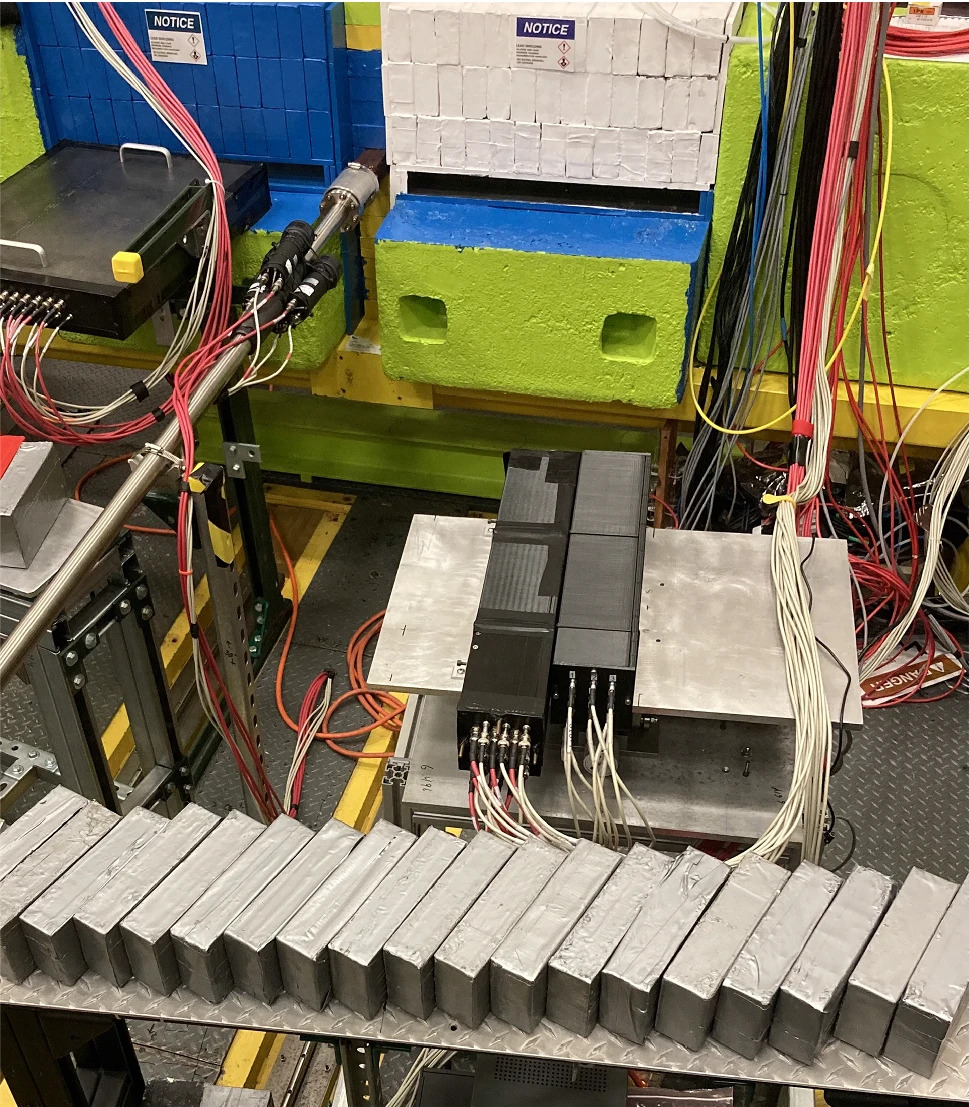
\includegraphics[width=0.5\textwidth]{3x3telescope.jpg}
    };
    \end{tikzpicture}
  \end{frame}
  %
  \begin{frame}{Raggi cosmici}
    
\begin{columns}[onlytextwidth,T]
  \begin{column}{.45\linewidth}
      \begin{itemize}
          \item Intensità muoni cosmici di \mbox{energia $\small>$\SI{1}{\GeV}} al livello del mare:
      $$
          I \sim 70\ m^{-2} s^{-1} sr^{-1}
      $$
          \item Contenuto di energia dei raggi cosmici:
      %\[
      $$
      1 - \SI{e10}{\GeV}
      $$
          \item Fonte di rumore per i rivelatori a scintillazione
      %\]
      \end{itemize}
  \end{column}
  %\begin{column}{.45\linewidth}
  %\end{column}
\end{columns}
    % create TikZ picture environment
    \begin{tikzpicture}[remember picture, overlay]
    \node[left=1.2cm] at (current page.east) 
    {
        \includegraphics[width=0.5\textwidth]{cosmo-cascade.png}
    };
    \end{tikzpicture}

  \end{frame}
  %
  \begin{frame}{Algoritmo di tagging di raggi cosmici}
      \begin{columns}[onlytextwidth,T]
      \begin{column}{.60\linewidth}
      \begin{itemize}
          \item Muone cosmico:
              \begin{itemize}
                  \item Traiettoria di angolo $\varphi \in [0°, 45°]$ \mbox{con la verticale}
                  \item Velocità $v \in [0.9, 1[\ c$
                \item Energia media $\small\sim$\SI{4}{\GeV}
              \end{itemize}
          \item Per ogni hit selezionata dal trigger L1 (seed), l'algoritmo verifica:
              \begin{itemize}
          \item Correlazione spaziale
          \item Correlazione temporale
              \end{itemize}
              con gli altri seed della stessa TS
      \end{itemize}
      \end{column}
      \begin{column}{.45\linewidth}
      \end{column}
    \end{columns}
    \begin{tikzpicture}[remember picture, overlay]
    \node[left=0.8cm] at (current page.east) 
    {
        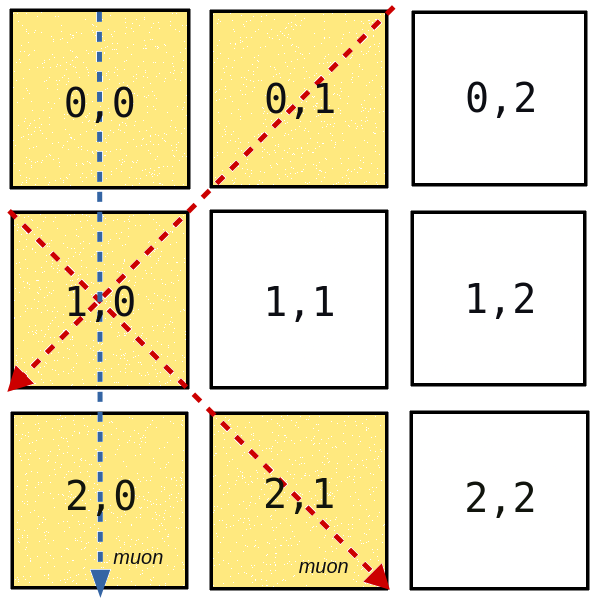
\includegraphics[width=0.4\textwidth]{3x3_side_indexes.png}
    };
    \end{tikzpicture}
  \end{frame}
  %
  \begin{frame}{Algoritmo di tagging di raggi cosmici - Correlazione temporale}
      \begin{columns}[onlytextwidth,T]
      \begin{column}{.45\linewidth}
          \lstinputlisting[basicstyle={\scriptsize\ttfamily},language=C++,frame=none]{../lst/time_corr.cpp}
      \end{column}
      \begin{column}{.45\linewidth}
      \end{column}
    \end{columns}
    \begin{tikzpicture}[remember picture, overlay]
    \node[left=0.8cm] at (current page.east) 
    {
        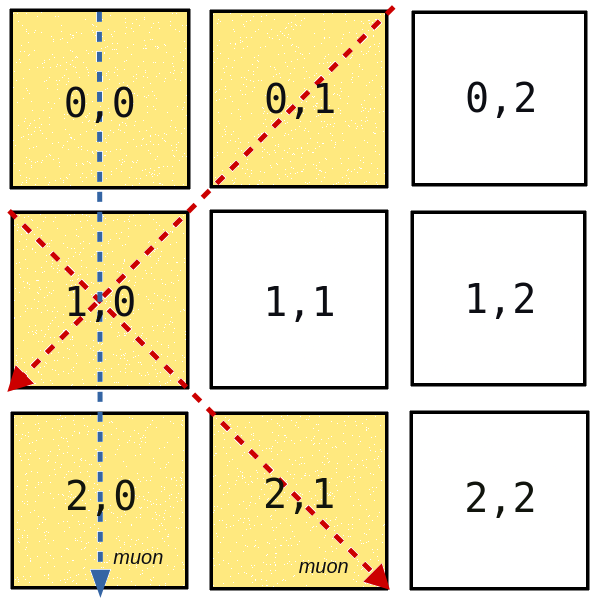
\includegraphics[width=0.4\textwidth]{3x3_side_indexes.png}
    };
    \end{tikzpicture}
  \end{frame}
  %
  \begin{frame}{Algoritmo di tagging di raggi cosmici - Correlazione spaziale}
      \begin{columns}[onlytextwidth,T]
      \begin{column}{.60\linewidth}
          Preso un elemento $e_{i,j}$\ , $a \coloneqq i + j$, $b \coloneqq i - j:$
\[
	d_a = \{ e_{i',j'} \mid i' + j' = a\}
\]
\[
	d_b = \{ e_{i',j'} \mid i' - j' = b\}
\]
%Gli elementi soprastanti $e_{i,j}$ compresi tra le due diagonali $d_a$ e $d_b$ sono definiti da
\[
	I_{up} = \{ e_{i',j'}\ \mid\ i' + j' \leq a\ \land\ i' - j' \leq b\}
\]
%Gli elementi sottostanti $e_{i,j}$ compresi tra le due diagonali sono definiti da 
\[
	I_{down} = \{ e_{i',j'}\ \mid\ i' + j' \geq a\ \land\ i' - j' \geq b\}
\]
La hit$_{i',j'}$ è correlata alla hit$_{i,j}$ se:
$$
          \begin{cases}
              \text{hit}_{i',j'} \in I_{up} & \text{\small {\footnotesize con} $\ t_{\text{hit}_{i',j'}} < t_{\text{hit}_{i,j}}$}\\ 
              \text{hit}_{i',j'} \in I_{down} & \text{\small {\footnotesize con}\ $\ t_{\text{hit}_{i',j'}} > t_{\text{hit}_{i,j}}$}
          \end{cases}
$$
      \end{column}
      \begin{column}{.45\linewidth}
      \end{column}
    \end{columns}
    \begin{tikzpicture}[remember picture, overlay]
    \node[left=0.8cm] at (current page.east) 
    {
        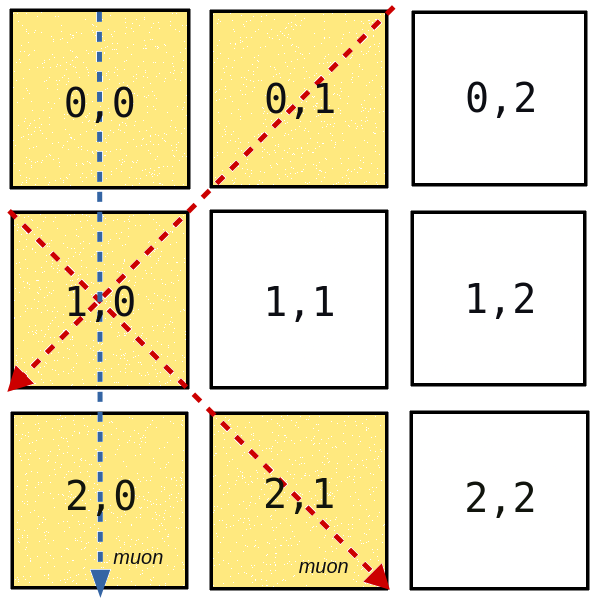
\includegraphics[width=0.4\textwidth]{3x3_side_indexes.png}
    };
    \end{tikzpicture}
  \end{frame}
  \begin{frame}{Strumenti di analisi e test}
      \begin{columns}[onlytextwidth,T]
      \begin{column}{.45\linewidth}
      \begin{itemize}
          \item Creazione grafici e istogrammi dai dati contenuti nei file prodotti da TriDAS 
          \item Ambiente di test per riprodurre l'intero sistema distribuito su una singola macchina usando docker compose
          \item Esecuzione offline dei trigger 
      \end{itemize}
      \end{column}
      \begin{column}{.45\linewidth}
      \end{column}
    \end{columns}
    \begin{tikzpicture}[remember picture, overlay]
    \node[left=0.8cm] at (current page.east) 
    {
        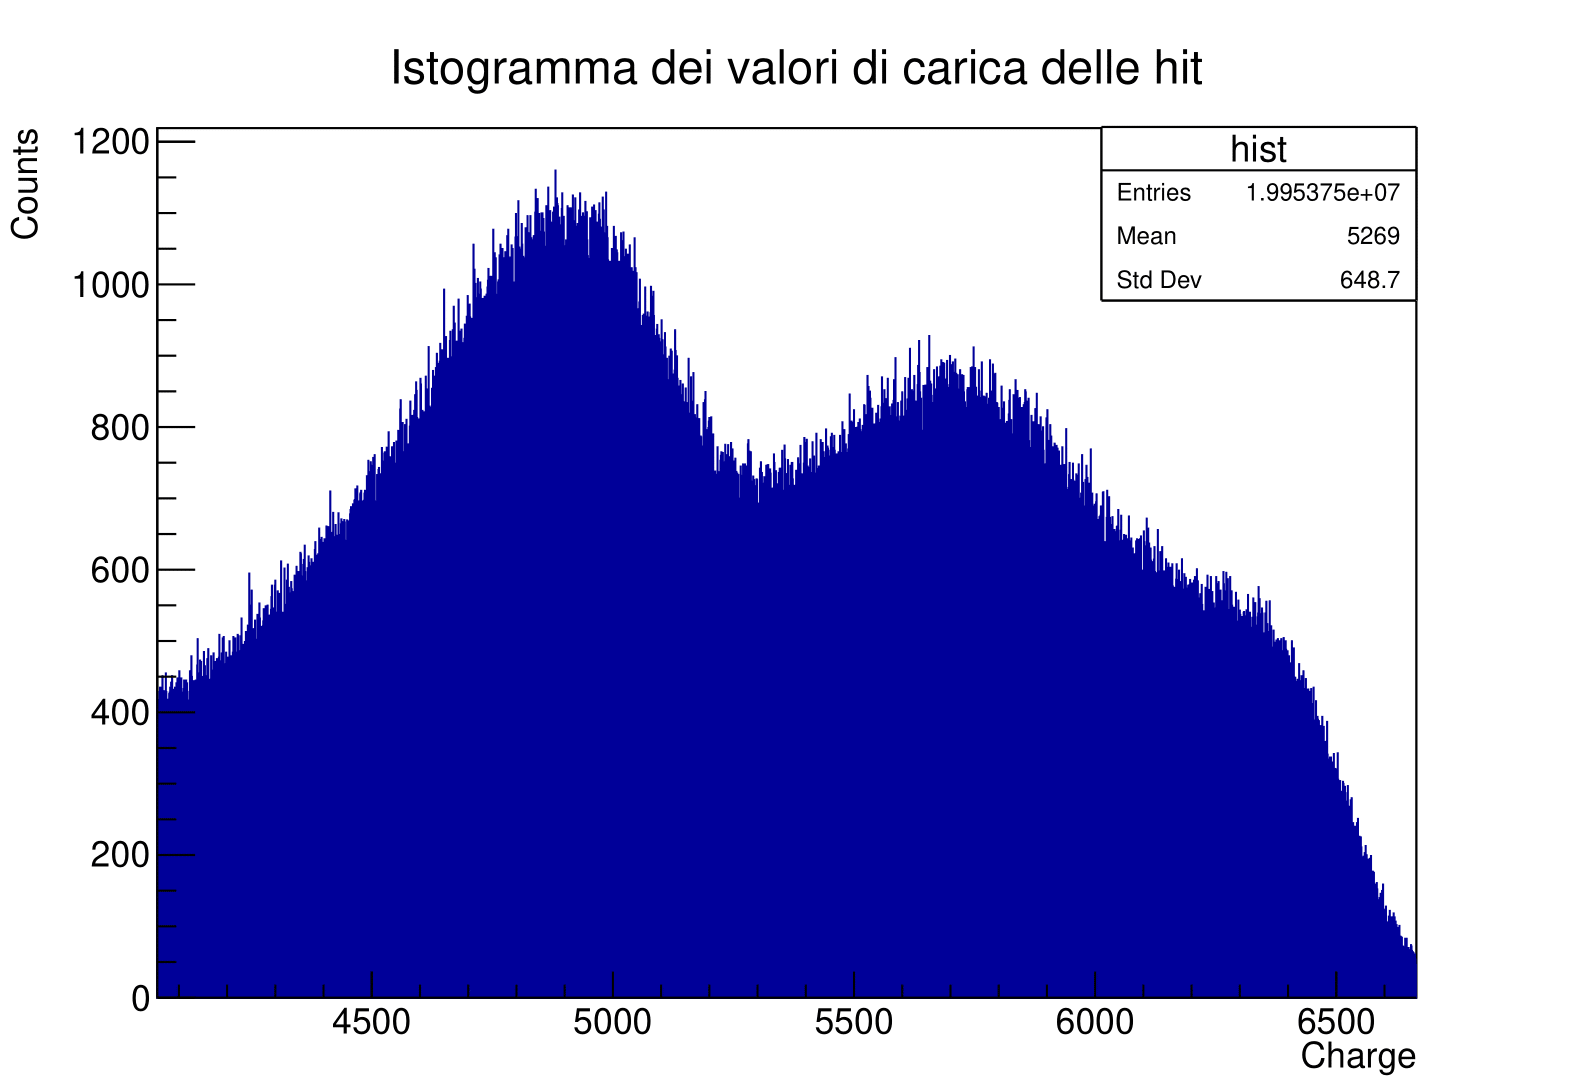
\includegraphics[width=0.50\textwidth]{c1-1.png}
    };
    \end{tikzpicture}
  \end{frame}
  \begin{frame}{Conclusioni}
      \begin{itemize}
        \item Algoritmo integrato con successo dentro l'ambiente di test di TriDAS come trigger L2
            \begin{itemize}
                \item Nonostante difficoltà nell'adattare la geometria a uno scenario diverso da quello per cui il sistema era pensato 
            \end{itemize}
        \item Necessario valutare l'impatto dei parametri dell'algoritmo sull'efficacia della selezione di eventi generati da raggi cosmici
      \end{itemize}
  \end{frame}
\end{document}
